\documentclass[class=article, crop=false]{standalone}
\usepackage[subpreambles=true]{standalone}
\usepackage{import}
\usepackage[T1]{fontenc}
\usepackage[utf8]{inputenc}
\usepackage[english, danish]{babel}
\usepackage{graphicx,wrapfig,lipsum}

\begin{document}
    Der blev benyttet ArrayList til at håndtere problematikken omkring de almindelige arrays, som har fixed længde, fordi man nødt til at sikre sig at der ikke kommer null pointers hvis det ikke er fyldt helt ud. ArrayList er en allerede implementeret klasse i java, mere specifikt i java.util-pakken. Her er ArrayList klassen smart, da den virker som et flexibelt array. Dette betyder, at når du tilføjer eller fjerner fra den vil dens længde tilpasse sig efter hvor mange elementer den indeholder.\par
    Brugen af ArrayLists kan simplificerer koden rimelig meget. Ser man f.eks. på Figur~\ref{fig:possibletobuildandsell} hvordan metoden “getCurrPlayerSquarePossibleToBuild(...)” tidligere har set ud, og hvordan “getCurrPlayerSquarePossibleToBuild(...)” ser ud nu, kan man se hvor meget funktionalitet ArrayList kan byde på.


    \begin{figure}[H]
        \centering
        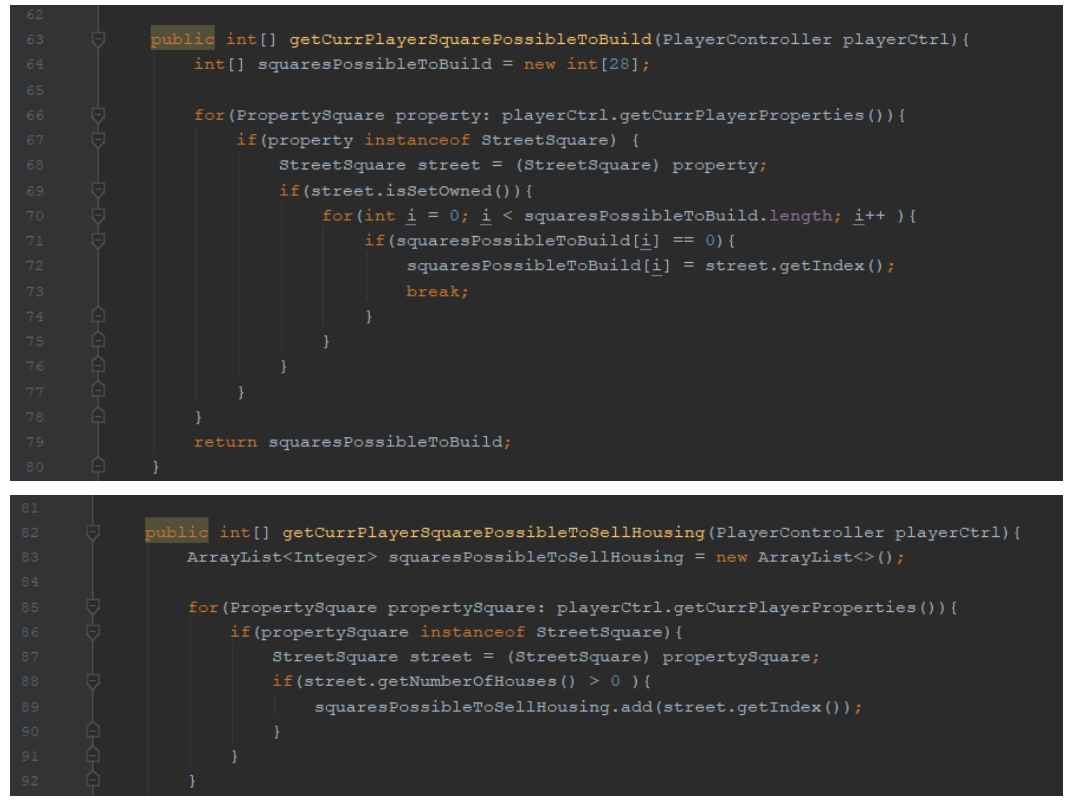
\includegraphics[scale=0.6]{pics/possibletobuildandsell}
        \caption{Kode over getCurrPlayerSquarePossibleToBuild og getCurrPlayerSquarePossibleToSellHousinng}\label{fig:possibletobuildandsell}
    \end{figure}
    \newpage
    Dog er den udleverede GUI ikke i stand til at bruge ArrayList i dens metoder, derfor er vi stadig nødt til at konvertere vores ArrayList om til et normalt array for at kunne vise dens indhold til brugeren (kan ses på Figur~\ref{fig:convert_arraylist}). Her kan vi dog relativt nemt oprette et nyt array ud fra størrelsen af vores ArrayList og derved antallet af objekter eller variable vi skal bruge pladser til, og derved ikke bekymrer os om null pointers i den array vi ender med.
    \begin{figure}[H]
        \centering
        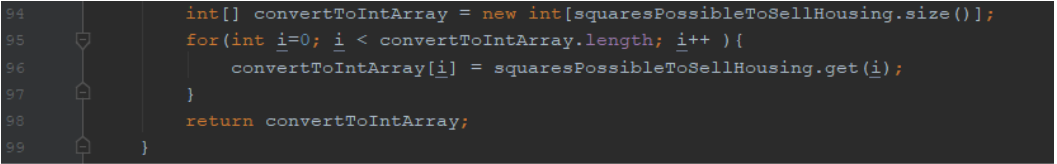
\includegraphics[scale=0.6]{pics/convert_arraylist}
        \caption{Kode over konvertering af ArrayList til almindelig array}\label{fig:convert_arraylist}
    \end{figure}


\end{document}